 
\chapter{Модель XY на динамических структурах c дальнодействием}
\label{ch:ch5}
В данной главе приведены результаты симуляции Монте-Карло  модели  XY на СБС с дальнодействием.  Показано возникновение фазового перехода первого порядка, подтверждаемое бимодальными распределениями энергии и анализом  кумулянтов Биндера. 


%Были проанализированы намагниченность, энергетические характеристики и их флуктуации в широком диапазоне параметров. Показано возникновение фазового перехода первого порядка, подтверждаемое бимодальными распределениями энергии и анализом Binder-кумулянтов, а также исследовано масштабное поведение наблюдаемых величин при увеличении длины цепи. Полученные данные количественно описывают коллективное магнитное поведение системы с длиннодиапазонными взаимодействиями и уточняют её критические свойства.
\section{3D} 
\subsection{Геометрический переход}



%\begin{figure}
%	\centering
%	\includegraphics[width=0.45\textwidth]{images/LI_XY_3D_r2_scale.png}
%	\caption{ }
%	\label{fig:xy_li_3d_r2scale}
%\end{figure}   


\subsection{Магнитный переход}

\textbf{Намагниченность}.  Для изучения режимов упорядоченности модели XY на СБС с дальнодействием рассмотрим величину намагниченности \eqref{xy_mean_magnetization}. 

Первый и второй моменты намагниченности  представлены на графике \ref{fig:xy_lr_mags}. По графикам полученным численным моделированием видно, что с ростом энергии межспиннового взаимодействия $J$ система стремится к упорядоченному режиму. При малом  $J$ системе соответствует  парамагнитная (неупорядоченная)  фаза. Углы спинов (значения $\theta_i$) спиновой конфигурации остаются случайными.

С увеличением энергии взаимодействия, кривые моментов намагниченности имеют резкий подъём обоих моментов в узком диапазоне  $J$, что соответствует переходу в упорядоченную фазу. Спины становятся сонаправленными. %а модуль намагниченности О(1). 
 %образуется дальняя корреляция по всей цепочке 
 
 Графики моментов намагниченности также показывают наличие эффекта конечного объема. С увеличением длины цепочки $N$  система достигает упорядоченного режима при меньшем  $J$. С ростом размера системы, переход становится более "резким" (случается в более узком интервале значений $J$). 

  \begin{figure}
	\centering
	\includegraphics[scale=0.30]{images/LI_XY_3D_m1_scale.png}
	\includegraphics[scale=0.30]{images/LI_XY_3D_m2_scale.png}
	%\includegraphics[scale=0.18]{Images/state_example2.png}
	\caption{ Первый и второй моменты намагниченности    \eqref{xy_mean_magnetization} как функции от  $J$ для цепочек длины $N=200; 300; 400$.     }
	\label{fig:xy_lr_mags}
\end{figure}

  \begin{figure}
	\centering
	\includegraphics[scale=0.30]{images/LI_XY_3D_e1_scale.png}
	\includegraphics[scale=0.30]{images/LI_XY_3D_e2_scale.png}
	%\includegraphics[scale=0.18]{Images/state_example2.png}
	\caption{ Первый и второй моменты  энергии на спин как функции от  $J$ для цепочек длины $N=200; 300; 400$.     }
	\label{fig:xy_lr_e}
\end{figure} 

\textbf{Энергия}. Рассмотрим график зависимости средней энергии на спин $\langle e \rangle = \langle H \rangle  / N $ \ref{fig:xy_lr_e}. 

При малом значении $J$ энергия около нулевая, так как область низкого взаимодействия соответствует парамагнитной (неупорядоченной) фазе, в которой ориентации спинов $\theta_i$ дезориентированы, а корреляции спинов  отсутствуют.    % $ <cos(thetai-thetaj) -> 0  $

С ростом $J$ система в среднем принимает состояния с наименьшей энергией. 
Аналогично моментам намагниченности, с ростом длины цепочки $N$, кривые энергии имеют более резкое  отрицательное падением в более узком диапазоне значений $ J$.  
 
 Резкое падение энергии и скачок намагниченности, зависящие от размера системы $N$ происходят примерно в одних и тех же интервалах $J$. 
 
 
 
 
 \subsubsection{Оценка кумулянтов Биндера и его ошибок}
 
 %Здесь пока, так как проблема с большими ошибками 
 %Мб переместится 
% 
% В течение моделирования системы c помощью Монте-Карло для фиксированных $N$ и $J$ сохраняются намагниченность  $m$ \eqref{xy_mean_magnetization},  энергия $e$,  квадрат радиуса вращения $R_g^2$, квадрат расстояния между концами БСП $R^2$.  Свойства конфигурации сохраняются каждый блок алгоритма, состоящий из $20 \times N^2$  локальных шагов \ref{subsection:snake} и одной смены соединений \ref{subsection:reconnect}. Таким образом сохраняется временной ряд для величин. % Автокоррелляци между которыми 
% 
%  Есть временной ряд для намагниченности ${ m_1, m_2, ..., m_i, ...}$. 
%  
%  
%  \begin {enumerate} 
%  \item Временной ряд делится на блоки ($blockSize=100$), по которым происходит усреднение для устранения автокорреляции между сохраненными величинами и считаются моменты намагниченности: $\{m_{b1}, m_{b2}, m_{b3}, ...\}$,  $\{m^2_{b1}, m^2_{b2}, m^2_{b3}, ...\}$,  $\{m^4_{b1}, m^4_{b2}, m^4_{b2}, ...\}$. 
% 
%   \item Из средних моментов по блокам получают итоговые моменты намагниченности:
%   $\langle m^2 \rangle = \frac{1}{N_{blocks}} \sum_{i=1}^{N_{blocks}} m^2_{bi}  $,    $\langle m^4 \rangle = \frac{1}{N_{blocks}} \sum_{i=1}^{N_{blocks}} m^4_{bi}  $.
%   
%   \item Получаем оценку для кумулянта биндера намагниченности: 
%   
%   $U_4 = 1 - \frac{\langle m^4 \rangle }{  3 \langle m^2 \rangle   }^2 $. 
%   
%     \item Далее оцениваем статистическую ошибку с помощью  бутстрэпа по блокам. Для этого генерируем $B= 100$ случайных выборок  блоков с возвращением той же длины, что и исходный набор блоков. Для каждой выборки оцениваем $U_4$ и получаем набор из $B$  оценок. В качестве статистической ошибки для кумулянта биндера берем размер интервала между перцентиль $q_{84}$ и $q_{16}$ --- это оценка интервала в одну $\sigma$. 
% 
%   \end{enumerate} 
% 
% 
% 
%  
% 
 

\subsection{Распределения}


 \begin{figure}
	\centering
	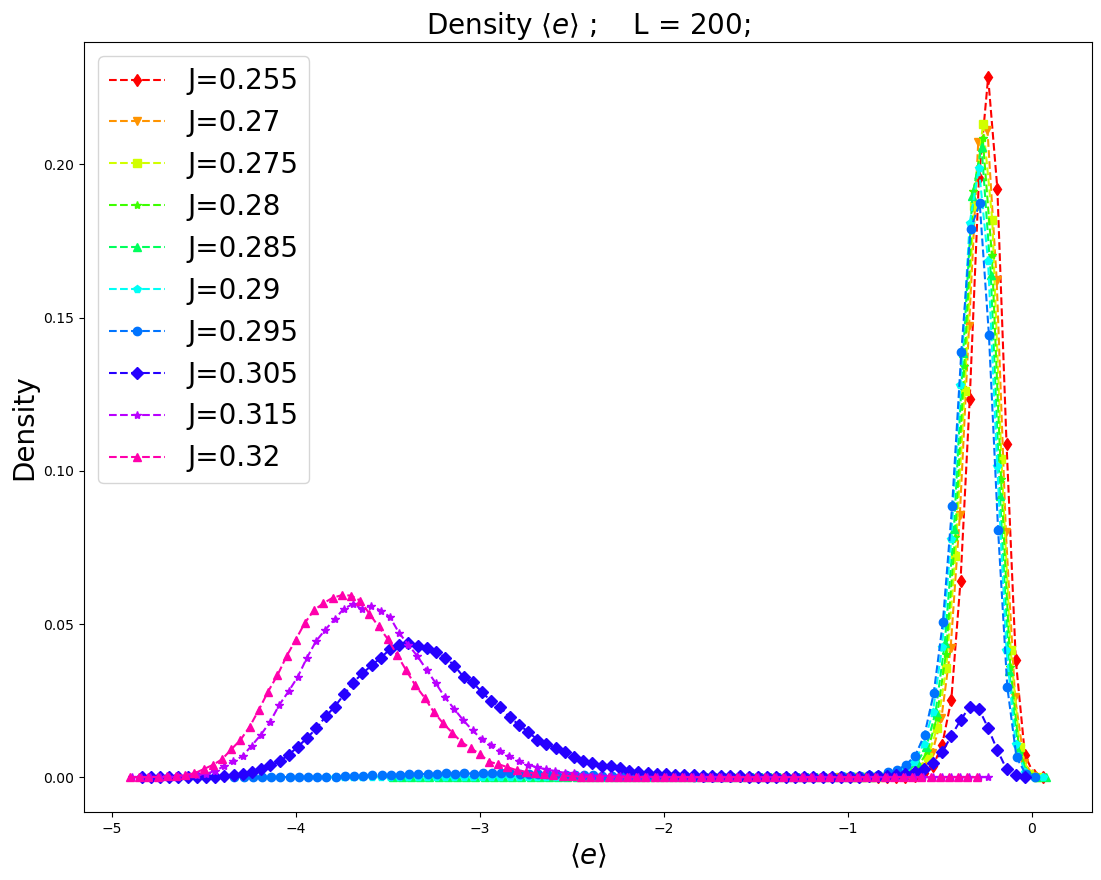
\includegraphics[scale=0.30]{images/distr_energy_200.png}
	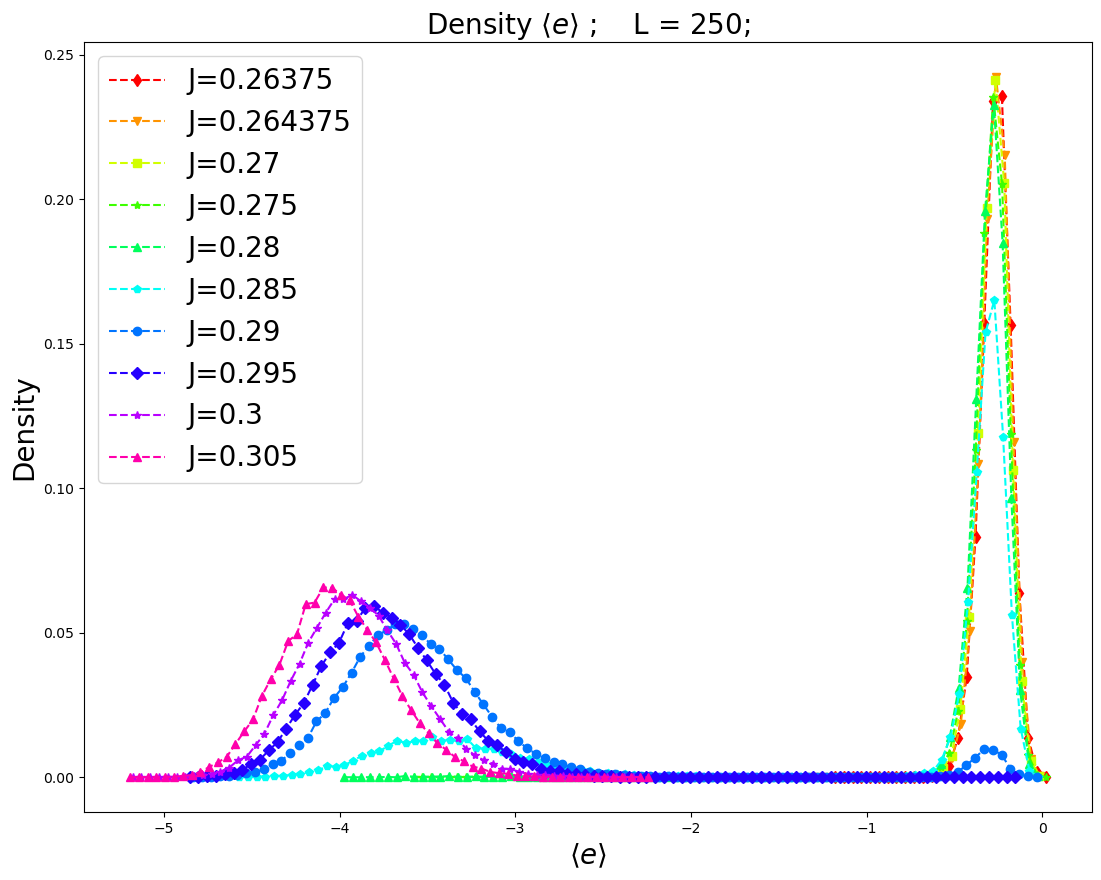
\includegraphics[scale=0.30]{images/distr_energy_250.png} \\ 
	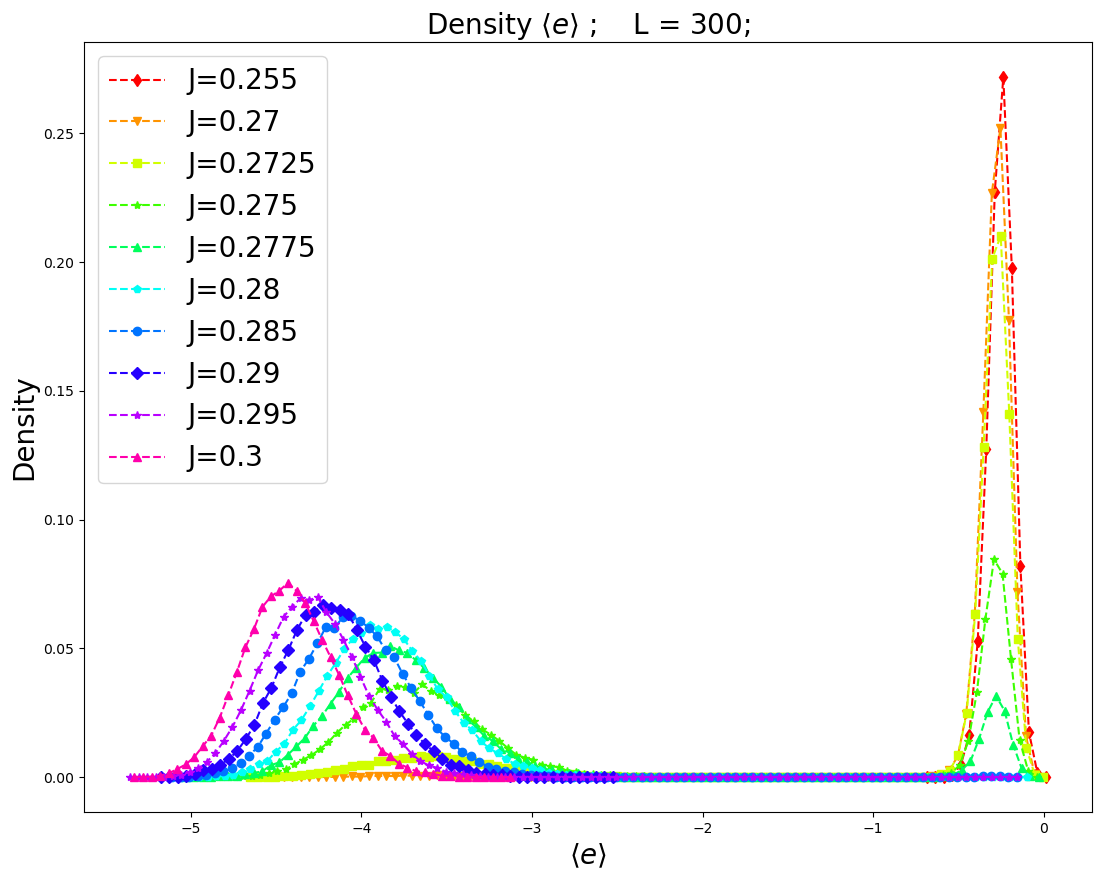
\includegraphics[scale=0.30]{images/distr_energy_300.png}
	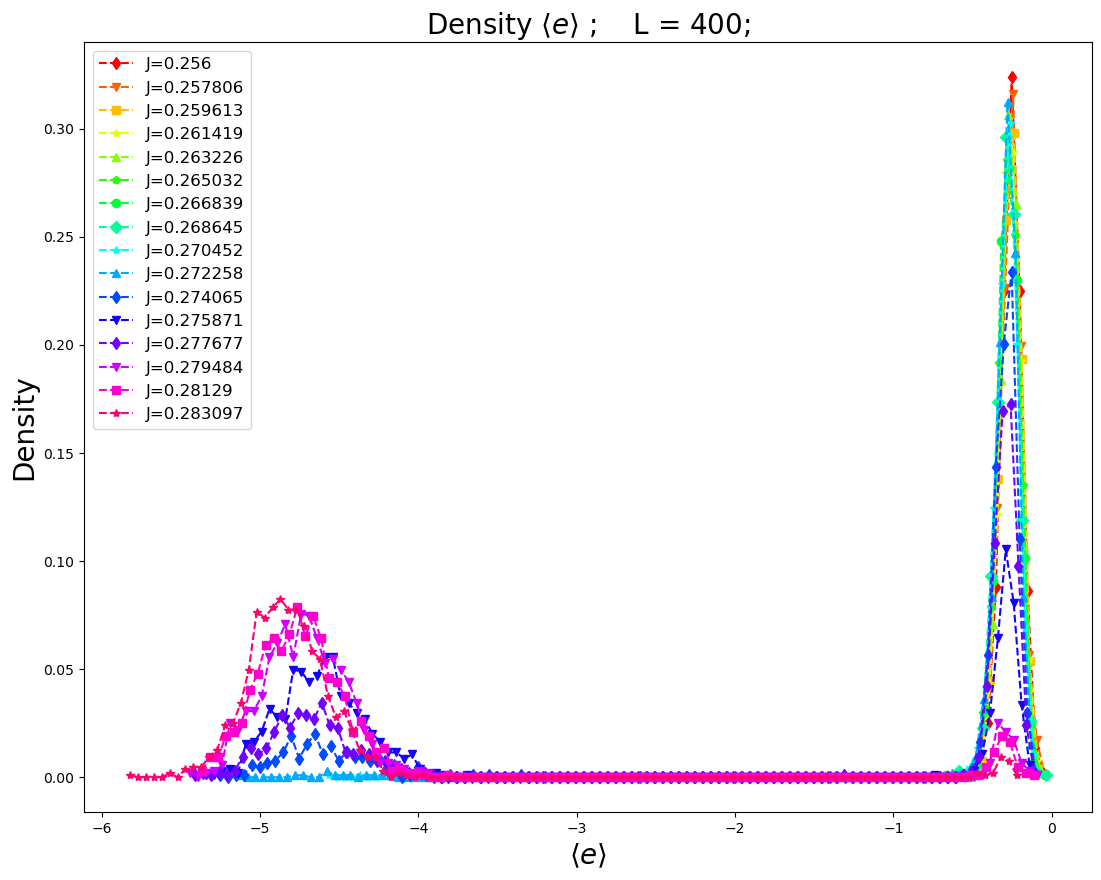
\includegraphics[scale=0.30]{images/distr_energy_400.png} 
	%\includegraphics[scale=0.18]{Images/state_example2.png}
	\caption{     }
	\label{fig:xy_lr_e_distr}
\end{figure} 



 \begin{figure}
	\centering
	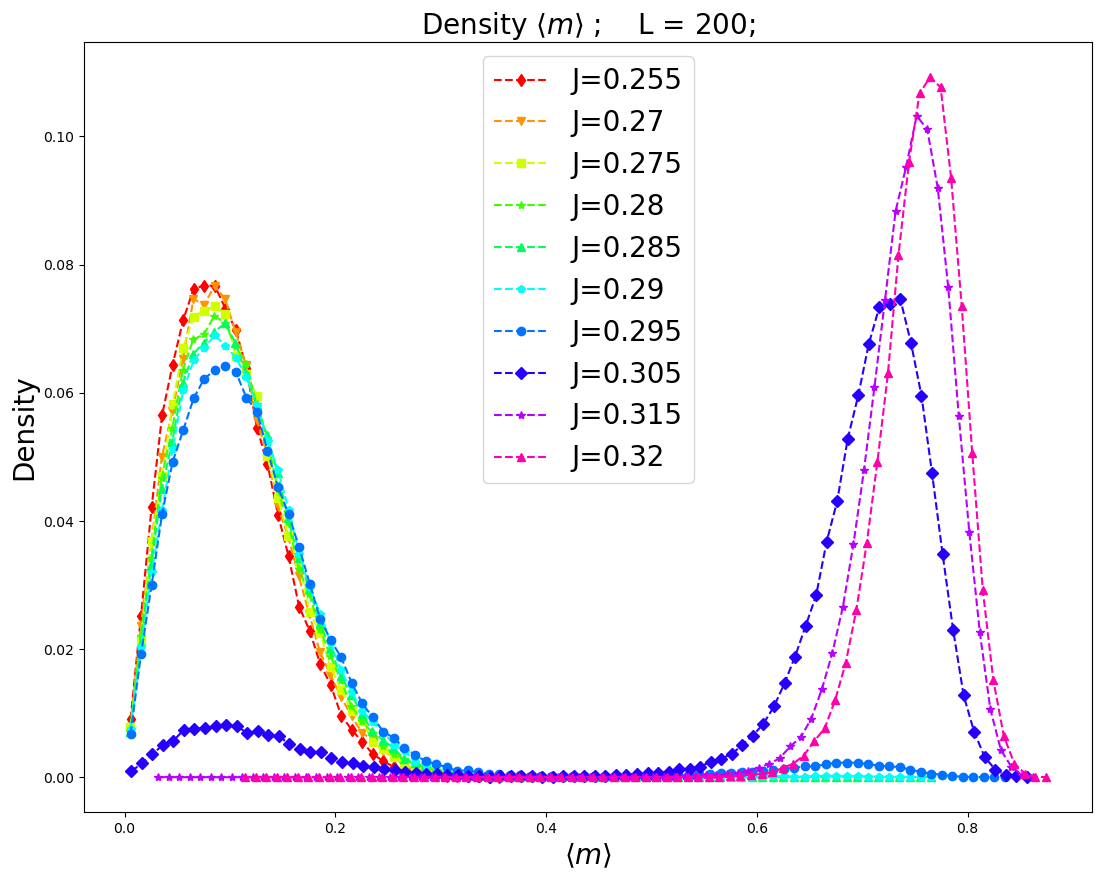
\includegraphics[scale=0.30]{images/distr_mags_200.png}
	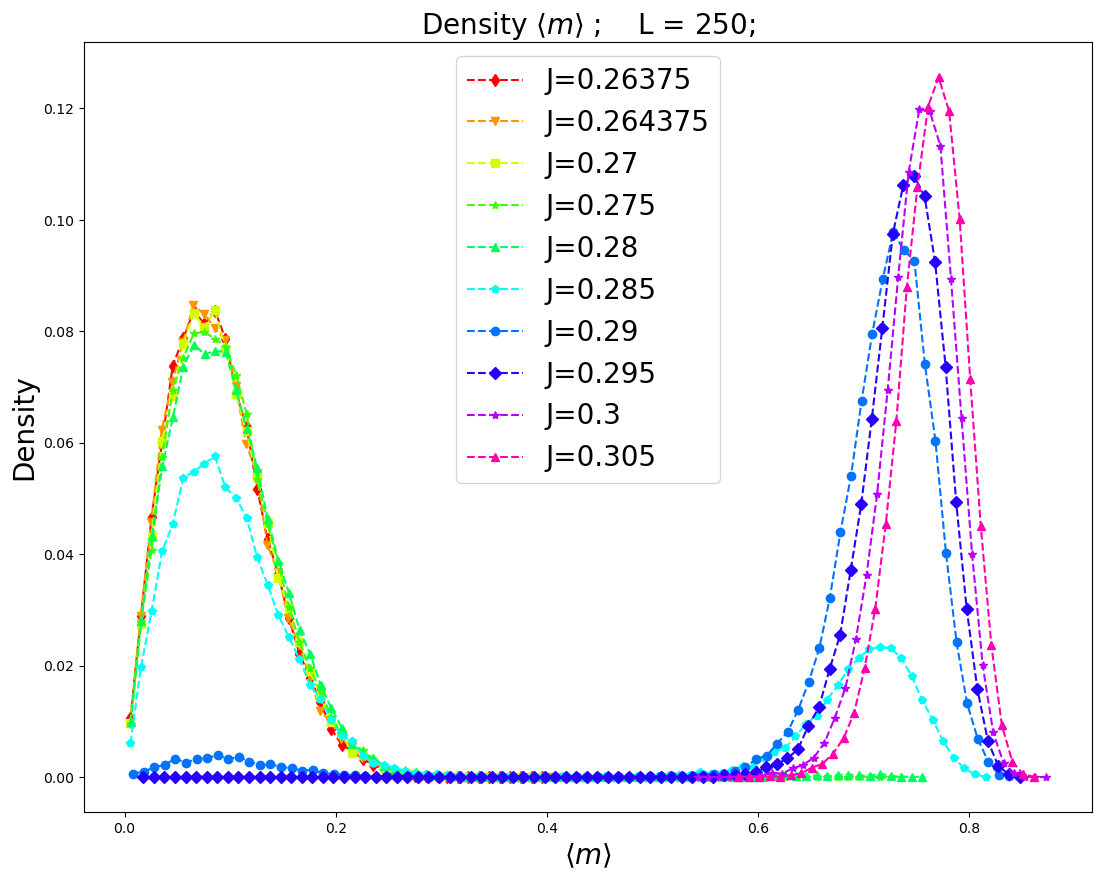
\includegraphics[scale=0.30]{images/distr_mags_250.png} \\ 
	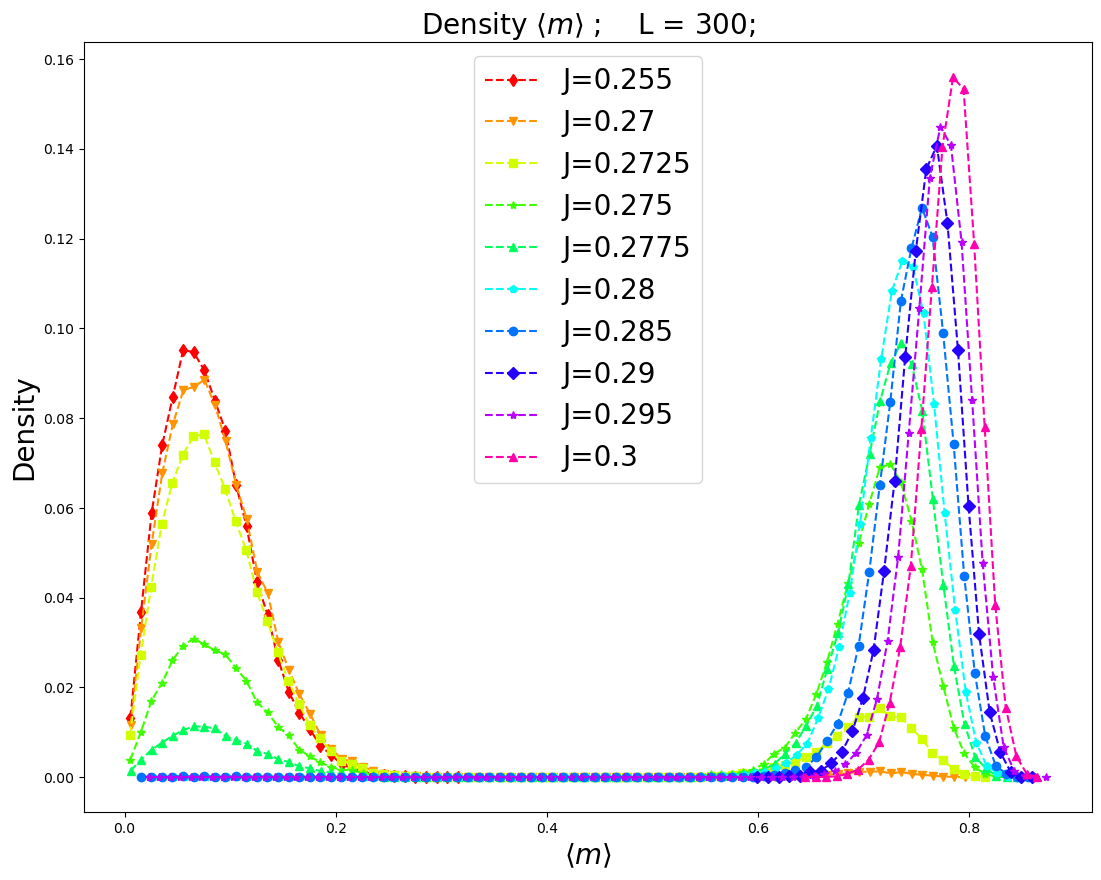
\includegraphics[scale=0.30]{images/distr_mags_300.png}
	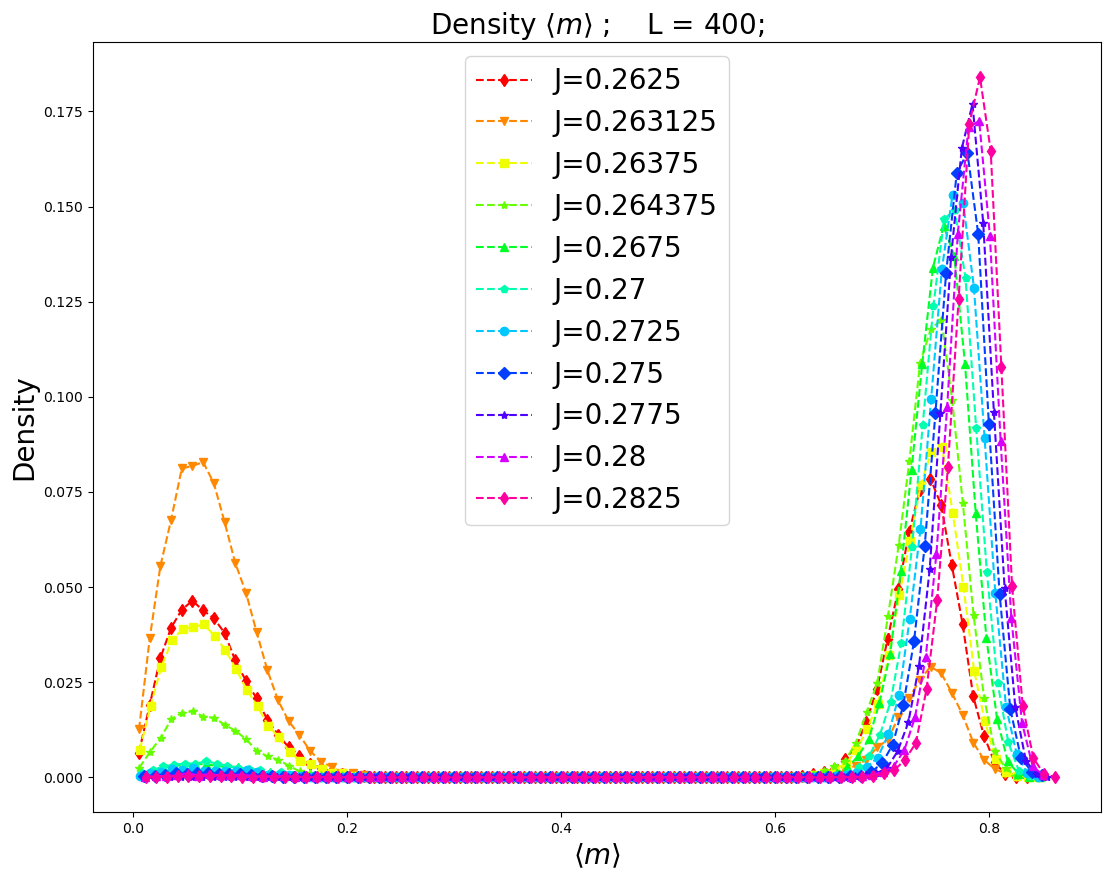
\includegraphics[scale=0.30]{images/distr_mags_400.png} 
	%\includegraphics[scale=0.18]{Images/state_example2.png}
	\caption{     }
	\label{fig:xy_lr_m_distr}
\end{figure}  





\begin{figure}
	\centering
	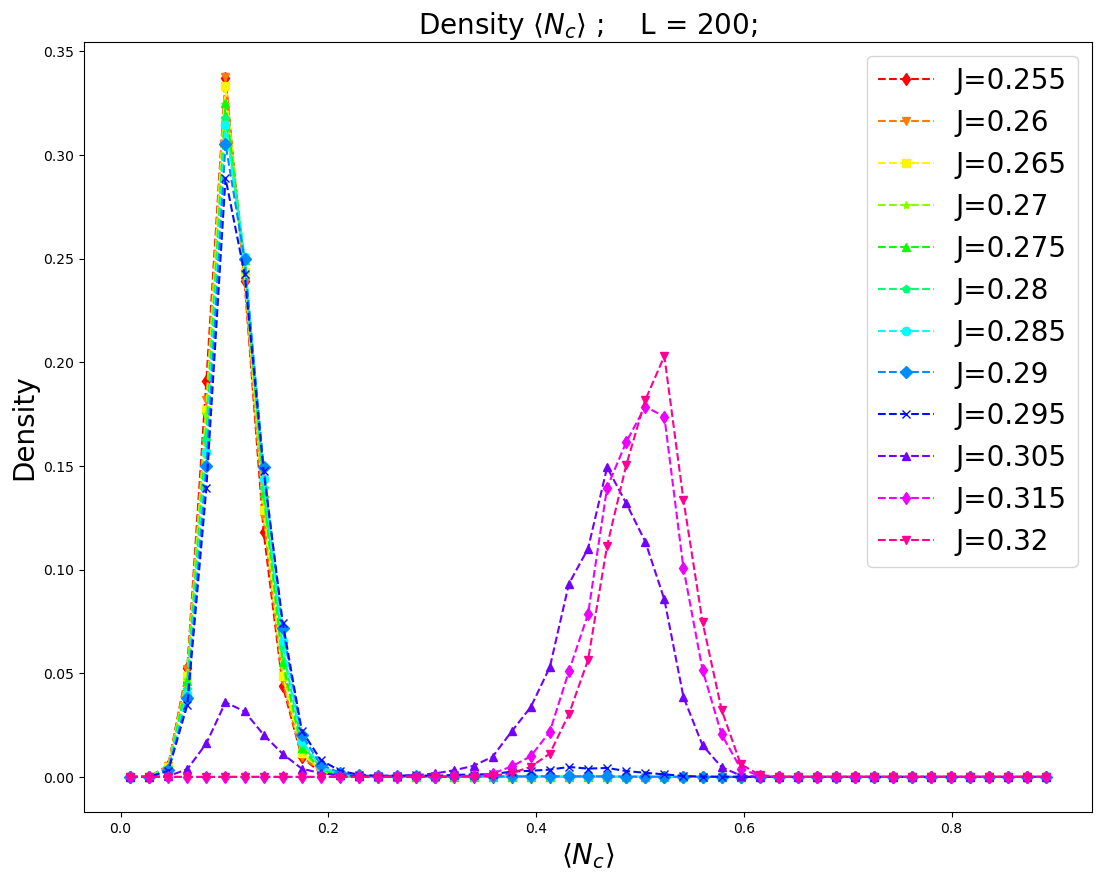
\includegraphics[scale=0.30]{images/distr_N_c_200.png}
	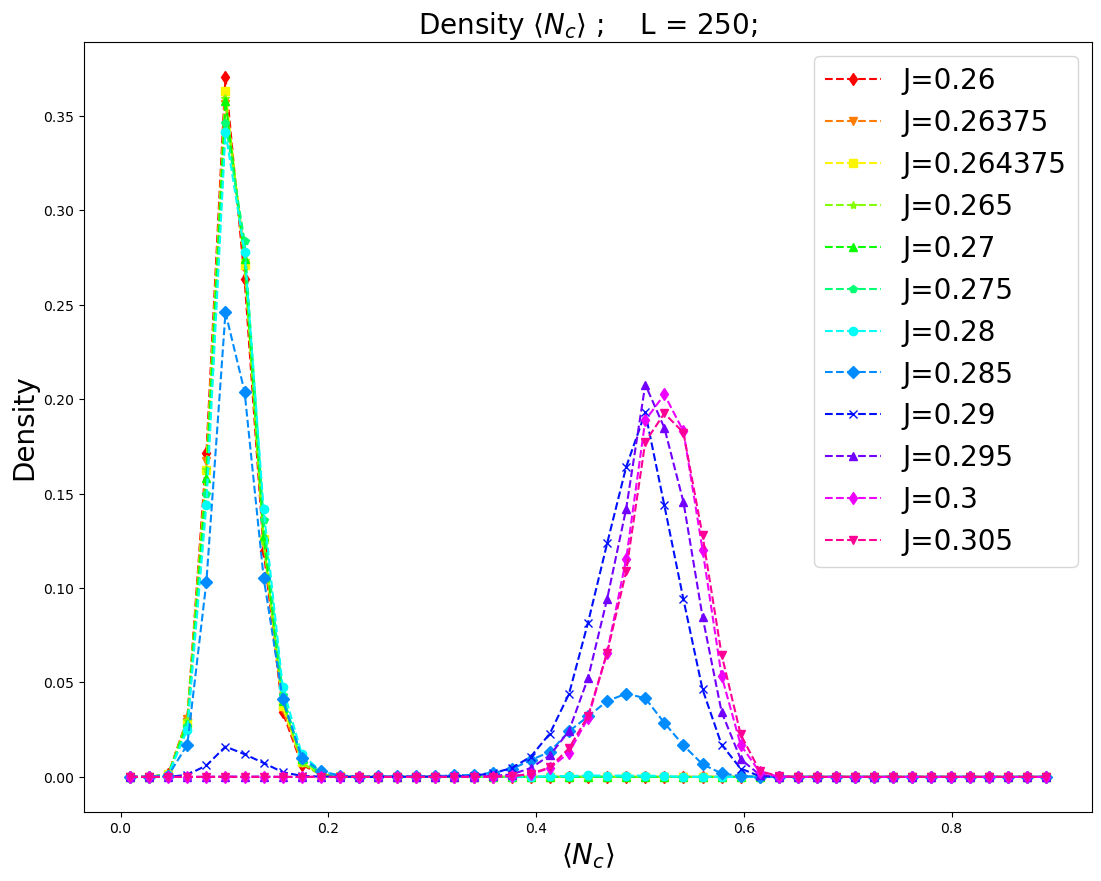
\includegraphics[scale=0.30]{images/distr_N_c_250.png} \\ 
	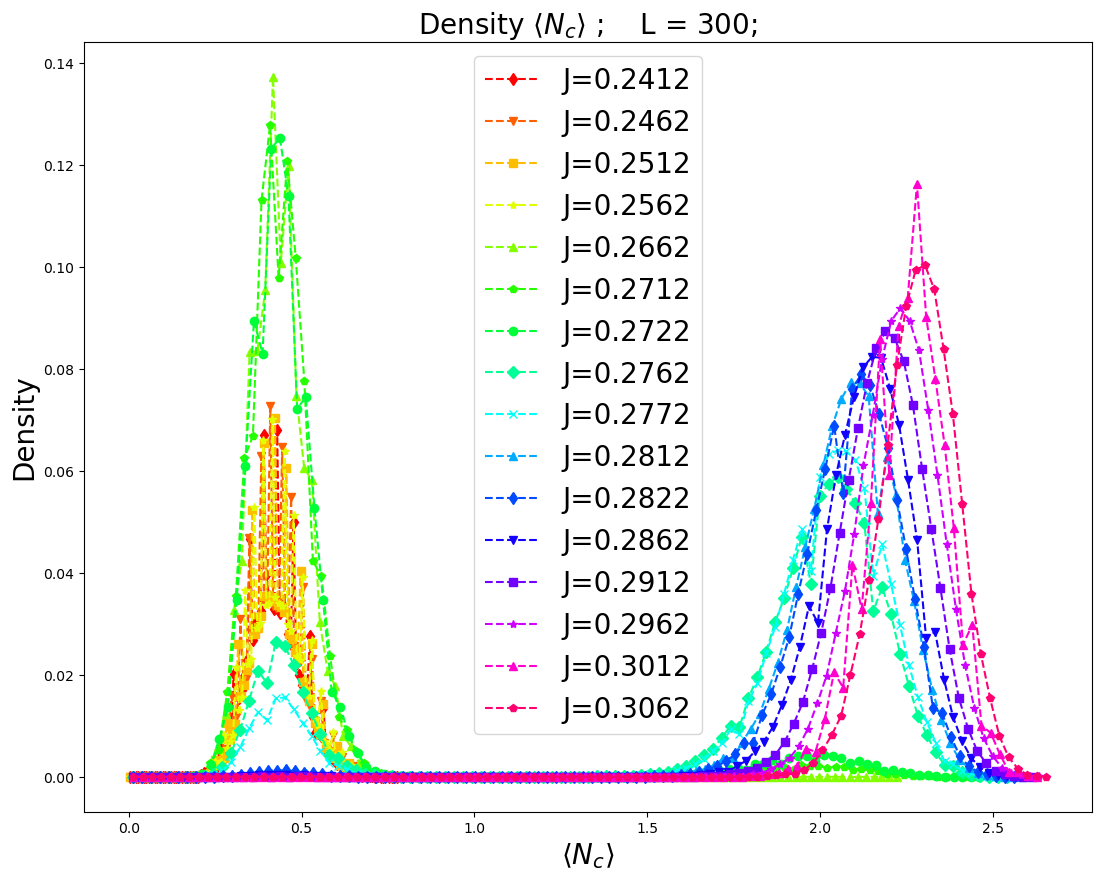
\includegraphics[scale=0.30]{images/distr_N_c_300.png}
	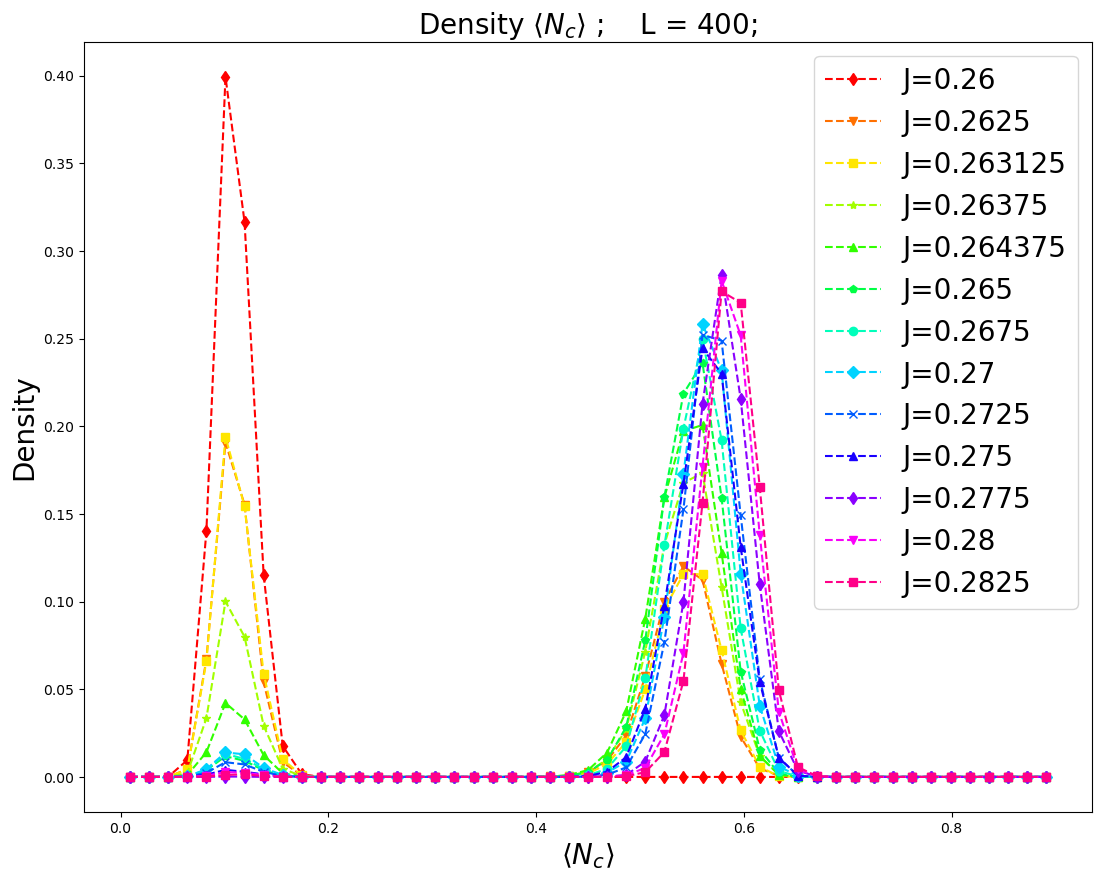
\includegraphics[scale=0.30]{images/distr_N_c_400.png} 
	%\includegraphics[scale=0.18]{Images/state_example2.png}
	\caption{     }
	\label{fig:xy_lr_Nc_distr}
\end{figure}   